\documentclass{beamer}

\usepackage{tikz}


\begin{document}
    \begin{frame}
        \centering
        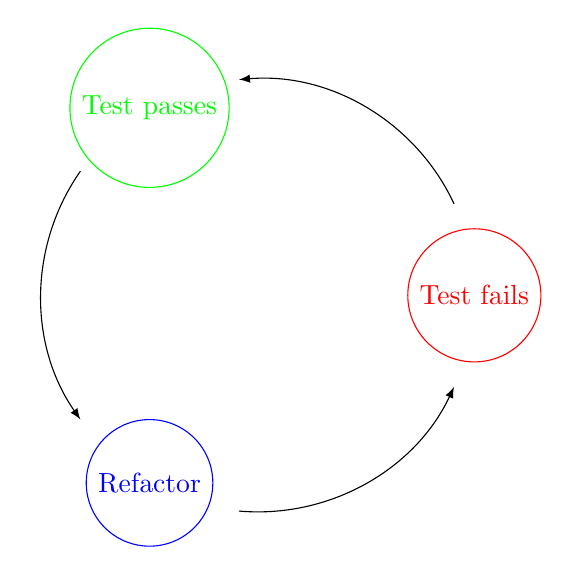
\begin{tikzpicture}
            \def \n {3}
            \def \radius {2.75cm}
            \def \margin {25}
            \foreach \s/\A/\C in {1/Test fails/red,2/Test passes/green,3/Refactor/blue}
            {
              \node[draw, circle,\C] at ({360/\n * (\s - 1)}:\radius) {\A};
              \draw[->, >=latex] ({360/\n * (\s - 1)+\margin}:\radius) arc ({360/\n * (\s - 1)+\margin}:{360/\n * (\s)-\margin}:\radius);
            }
            \end{tikzpicture}
    \end{frame}
\end{document}